%!TEX root = P231_notes.tex
\section{Green's Functions from Statistics and Gaussian Integrals}

In Section~\ref{sec:CHO:fields} we showed how fields emerge from a system of nearest-neighbor coupled harmonic oscillators. To leading order, fields are described by the wave operator. We remarked that the differential equation that governs a physical theory comes from a variation of the action functional $\delta S[\varphi]=0$. We even motivated how one builds theories: you start by imagining the most general action $S$ and then you remove terms because they violate symmetries or because they're suppressed by an energy scale $M$ much larger than the energy $E$ or physical phenomena you're examining. The latter point amounts to a $(E/M)^n$ suppression on physical observables. 

At this point, you may ask: well, where does $\delta S = 0$ come from? Curious, aren't we? It turns out that this connects to a few different ideas which we'll map out in this section. In case you haven't noticed, the latter part of these notes are much less technical than the first half. The point is no longer to teach you techniques. We are stepping back and seeing how these ideas interconnect with different theoretical structure that you may [soon] know. Don't worry if there are more results that are left to you to prove or look up, the goal isn't the technical derivation. The goal is to see the interconnection of these tools.

In this section, we'll make a connection to a bit of probability theory and a cute trick for solving Gaussian integrals. First, though, a quantum mechanical interlude.

\subsection{Quantum Mechanics: Green's Function from the Path Integral}

Time evolution by some amount of time $\Delta t$ in quantum mechanics is enacted by the Hamiltonian (energy) as an operator: $e^{i\hat H\Delta t}$. This time evolution may be described as a Green's function that takes an initial state $\Psi(q_0,t_0)$ and evolves it into a final state $\Psi(q, t)$. The wavefunctions are defined by a projection of a state $|\psi(t)\rangle$ onto the position basis $q$:
\begin{align}
	\Psi(q,t) = \langle q | \psi(t) \rangle \ .
\end{align}
Since $|\psi(t)\rangle$ is the time evolution of $|\psi(t_0)\rangle$ by a time $\Delta t = t-t_0$, we may continue:
\begin{align}
	\Psi(q,t) 
	&= \langle q | e^{-i\hat H \Delta t} |\psi(t_0) \rangle
	\\
	&= \int dq_0\langle q | e^{-i\hat H \Delta t} |q_0 \rangle\langle q_0 |\psi(t_0) \rangle 
	\\
	&= \int dq_0\,\langle q | e^{-i\hat H \Delta t} |q_0 \rangle \Psi(q_0, t_0)
	\ ,
\end{align}
where we have simply inserted a complete set of states (\emph{multiplied by one}) $\mathbbm{1} = \int dq_0 |q_0 \rangle\langle q_0 |$; this is simply the completeness relation that we recall from our review of linear algebra. We identify the quantity $\langle q | e^{-i\hat H \Delta t} |q_0 \rangle$ as the Green's function $G(q,t;q_0,t_0)$ since it now manifestly plays the role of a Green's function to solve for the state $\Psi(q,t)$ given the initial state $\Psi(q_0, t_0)$:
\begin{align}
	\Psi(q,t)\, 
	&= \int dq_0\, G(q,t;q_0,t_0) \Psi(q_0, t_0)
	\ . 
\end{align}
We didn't have to explicitly write the Schr\"odinger equation because that's already implicit in our starting point that $e^{-i\hat H \Delta t}$ is the time-evolution operator. 

If you go over the path integral formulation of quantum mechanics, one finds that by repeating this trick and inserting a complete set of states over \emph{many} time slices between $t_0$ and $t$ you end up with\footnote{You may refer to the first couple of lectures here: \url{https://sites.google.com/ucr.edu/p230b/}} a closed form expression for the Green's function:
\begin{align}
	G(q,t;q_0,t_0)  = \int \mathcal Dq(t) \, e^{iS[q]/\hbar} \ .
	\label{eq:G:QM}
\end{align}
\begin{exercise}
For those with some familiarity with quantum mechanics, derive the above result. Be sure to keep track of how $e^{i\hat H t}$ turns into $e^{iS[q]}$. I personally find this to be the most compelling motivation for defining the action $S$ as the difference of the kinetic and the potential energies. Hint: you can slice up the finite time interval $t$ into a bunch of tiny time slices $\varepsilon t$. You can use the following matrix/operator relation: $e^{\varepsilon(A+B)} = e^{\varepsilon A}e^{\varepsilon B}+\mathcal O(\varepsilon^2)$ to separate out the kinetic and potential terms. Note that the kinetic terms depend only on momentum while the potential terms depend only on position. You can insert complete sets of momentum states, $\mathbbm 1 = \int dp |p\rangle \langle p|$ (check the normalization) and use $\langle q|p\rangle \sim e^{ipq}$, subject to conventions.
\end{exercise}
I've broken my usual convention of natural units and explicitly written out the $\hbar$ required to make $S[q]$ dimensionless. Recall that $[L]$ is energy and $S = \int dt \, L$ so that $[S] = E\times t$, which just happens to be the units of $\hbar$. The curious integration measure $\mathcal Dq(t)$ is an integral over different functions $q(t)$. The meaning is clear if we discretize in time:
\begin{align}
	\mathcal D q(t) = dq(t_0)\,dq(t_1)\,dq(t_2)\,\cdots dq(t_{N-1})\,dq(t_N = t) \ .
\end{align}
In other words, for each discrete time $t_i$, we vary the position $q(t_i)$ independently of the other positions. In this way, the integral over $\mathcal D q(t)$ is an integral over all possible functions $q(t)$ subject to the initial and final states.

You should interpret this expression as the famous quantum mechanical \emph{sum over histories}. The amplitude for a state to go from $\Psi(q_0,t_0)$ to $\Psi(q,t)$ includes a sum over the amplitude for each possible way to transition from the initial to the final state. At this point, you should recall the double slit experiment\footnote{The argument goes like this: imagine a double slit experiment. Now poke a third slit through the board; you sum over three paths. Now insert another board with two slits; you sum over $3\times 2 = 6$ paths. Now poke more holes, add more boards until you have an infinite number of boards each with an infinite number of holes. This corresponds to summing over all possible continuum paths from the initial to the final positions.}.
%
Evidently the quantity $e^{iS/\hbar}$ is the weight of each path. It corresponds to the amplitude of each path we're summing together. The total amplitude is given by the sum of these complex numbers with unit magnitude\footnote{You may want to look up `phasor' diagrams to see how to interpret this sum. Feynman describes this well in his for-the-public book \emph{QED: The Strange Theory of Light and Matter}, or you can see a more recent pop physics summary from PBS Spacetime: \url{https://youtu.be/vSFRN-ymfgE}.}.

$\hbar$ is also a measure of `quantumness'. Recall that it shows up in statistical mechanics due to the Gibbs paradox. The `quantum' of quantum mechanics refers to the fact that $\hbar\neq 0$ so that $[\hat p, \hat q] \neq 0$. As $\hbar\to 0$ one recovers the classical limit. We see that in the classical limit, the argument of the exponential $e^{iS/\hbar}$ becomes large and highly sensitive to variations of $S$. At this point one can make the \emph{saddle point approximation}. This is the observation that for $\hbar\to 0$, changes in $S[q]$ coming from nearby paths will rapidly change the phase of $e^{iS/\hbar}$ and cause the contributions of these nearby paths to cancel as one integrates over paths $q(t)$. There is one exception: when $S[q]$ is near an extremum (say, a minimum) then the contribution from nearby paths will change more slowly---this is obvious, you're at an extremum so the functional $S[q]$ is flat---and the those paths will dominate the integral. The result is that in the classical limit, the paths $q(t)$ that give the dominant contribution are simply those which realize an extremum of the action:
\begin{align}
	\delta S[q] = 0 \ .
\end{align}
And there you go, we have `derived' the principle of least action as the classical limit of time evolution in quantum mechanics. 

\begin{exercise}
How do you expect the Green's function \eqref{eq:G:QM} to change when we go from a \emph{particle} at $q(t)$ at time $t$ to a \emph{field} $\varphi(x,t)$ that takes in position $x$ and time $t$ as variables?  Congratulations, you're on your way to quantum field theory. 
\end{exercise}

\subsection{A probability refresher}

Now you may have a bit of mental whiplash as I change gears completely, but humor me a moment, we'll get back to the quantum mechanical picture shortly. 

A probability distribution function is an integrand $p(x)dx$ that tells you about the probability for some quantity $x$ to take some value. $p(x)$ is an infinitesimal probability defined by the statement that the probability for $x$ to take values within $x$ and $(x+dx)$ is $p(x)dx$. The probability for $x$ to take a value within some finite range $x\in[a,b]$ is
\begin{align}
	P(x\in[a,b]) = \int_a^b dx\, p(x) \ .
\end{align}
As you can expect, distributions are normalized so that
\begin{align}
	\int_{-\infty}^{\infty} dx\, p(x) = 1 \ .
\end{align}
A surprising amount of physics boils down to probability distributions. This shows up because we often deal with thermal/statistical uncertainty in condensed matter systems, data uncertainty in observational and experimental fields, and quantum uncertainty in anything `small.' Often you get multiple kinds of uncertainty\footnote{There's also the notorious `theory' uncertainty which is a statement about us not knowing what we don't know.}. Physics trains us to be skeptics. This is also part of what makes research-level training in physics so valuable in many other fields like machine learning or finance\footnote{It's almost surprising that this hasn't translated into fields like government and policy, though I suspect that this may be due to aspects that are lacking from a traditional physics training.}.

\begin{example}
The most famous distribution is the Gaussian:
\begin{align}
	g(x) &= \frac{1}{\sqrt{2\pi \sigma^2}} e^{\frac{-(x-\mu)^2}{2\sigma^2}} \ .
\end{align}
This is a distribution with mean $\mu$ and standard deviation $\sigma$. It is relevant for us in this course because up to pre-factors, it is an exponential of a quadratic polynomial---this looks similar to $e^{iS}$, where we argued that the quadratic parts of $S$ correspond to terms that give linear differential equations.
\end{example}

A probability distribution can be decomposed into moments. This the same way that you can decompose a finite mass distribution into \emph{moments} of inertia or the way that we can decompose a charge distribution into monopoles, dipoles, quadrupoles, etc. The $n^\text{th}$ moment of a distribution $p(x)$ is
\begin{align}
	M_n = \int_{-\infty}^\infty dx \, x^n p(x) \equiv \langle x^n \rangle \ .
\end{align}
The notation should remind you of a `correlation function' or an `expectation value.' The moments are an expansion that encode the whole distribution. There is, in turn, a fancy way to encode the moments in a \textbf{generating function}:
\begin{align}
	Z(J) \equiv \int dx\, e^{\xi x} \, p(x) \  
	= \langle e^{J x}\rangle
	= \langle 1 \rangle + J \langle x\rangle
	+ \frac{1}{2}J^2 \langle x^2\rangle + \cdots \ ,
	\label{eq:generating:function}
\end{align}
where $\xi$ is the argument of the generating function. The moments of the distribution are derivatives of the generating function:
\begin{align}
	M_n =
	\left.\frac{\partial^n Z(J)}{\partial J^n}\right|_{J = 0} \ .
\end{align}
The generating function is a \emph{Laplace transform} of the distribution $p(x)dx$. Like the Fourier transform, this is an integral transform that can be used to solve differential equations. To the best of my limited experience, engineers learn about Laplace transforms and physicists learn about Fourier transforms\footnote{I suspect this is because the momentum basis has physical significance for us. Maybe engineers are a little more skeptical of imaginary numbers than we are. Who knows. ... okay, I suspect someone with a mathematical background knows and will say that both physicists and engineers are being silly. \url{https://xkcd.com/435/}}.
\begin{example}
One could also write the Fourier transform of the distribution $p(x)dx$. This is called the \textbf{characteristic function} and is defined by
\begin{align}
	\phi(k) = \int_{-\infty}^\infty dx\, e^{ikx}p(x) = 1 + ikM_1 + \cdots \ .
\end{align}
Note that one can then write the distribution as
\begin{align}
	p(x) &= \int \dbar k\left( 1+ikM_1 + \frac{(ik)^2}{2!}M_2 + \cdots \right)e^{-ikx} \ ,
\end{align}
where the $e^{-ikx}$ looks like a $\delta$-function in momentum space. This is a toy version of the partition function in quantum field theory and the $\delta$-function imposes overall momentum conservation on any scattering process. 
\end{example}

\subsection{A cute trick: the Gaussian integral}

One of the neat things that you can show off to any young family members is the Gaussian integral. Removing annoying prefactors, one could imagine asking a high school student to integrate the Gaussian:
\begin{align}
	G = \int_{-\infty}^\infty dx\, e^{-\frac{1}{2}x^2} \ .
\end{align}
The exponent is supposed to be easy to solve, but the argument is quadratic. A change of variables doesn't help. What can we do?

It turns out we can simplify the problem by solving it in two dimensions. We may write $G^2$ as a two dimensional integral over independent variables:
\begin{align}
	G^2 = \int dx\, dy\, e^{-\frac{1}{2}(x^2 + y^2)} \ .
\end{align}
The trick is to pass to polar coordinates:
\begin{align}
	G^2 &= 2\pi \int_0^\infty\, r\,dr\, e^{-\frac{1}{2}r^2}
	\\
	&= 2\pi \int_0^\infty\, dw\, e^{-w}
	\\
	&= 2\pi \ . \label{eq:gaussian:integral}
\end{align}
From this we deduce that $G = \sqrt{G^2} = \sqrt{2\pi}$. This is a cute parlor trick that may earn you a tip of the hat in the right company. But we're not done yet; let's squeeze this parlor trick for all that it's worth.

\subsection{Down the Gaussian rabbit hole}

The action appears in our quantum Green's function \eqref{eq:G:QM}. We've identified something special about the quadratic part of the action: it gives linear differential equations. What can we learn about the nature of the Green's function from the Gaussian integral?

\paragraph{Gaussian with a prefactor.} The following generalization of the Gaussian integral should be `obvious' for you:
\begin{align}
	\int_{-\infty}^{\infty}dx\, e^{-\frac{1}{2}ax^2}
	&=
	\sqrt{\frac{2\pi}{a}} \ .
	\label{eq:gaussian:a}
\end{align}
This is `obvious' from dimensional analysis. Imagine giving $x$ some dimension ($x$-ness). In order for the argument of the exponential to be dimensionless, $a$ must carry dimension $[a]=-2$ of $x$-ness. The total integral has $x$-ness dimension $[G]=1$, from which we deduce that $[G]\sim 1/\sqrt{a}$. However, since the result must match \eqref{eq:gaussian:integral}, we know the proportionality.

\paragraph{Gaussian with a source.} Now consider generalizing further by adding a linear term. In field theory we call this a \emph{source} of $x$ because terms like this will give the right-hand sides (the source terms) of our differential equations. The result is:
\begin{align}
	\int_{-\infty}^{\infty}dx\, e^{-\frac{1}{2}ax^2 + Jx}
	&=
	\sqrt{\frac{2\pi}{a}}  e^{J^2/2a} \ .
	\label{eq:gaussian:with:source}
\end{align}
\begin{exercise}
Prove \eqref{eq:gaussian:with:source} by completing the square and changing variables. Use:
\begin{align}
	-\frac{1}{2}ax^2 + Jx = -\frac{1}{2}a\left(x-\frac{J}{a}\right)^2 + \frac{J^2}{2a} \ .
\end{align}
\end{exercise}

Note that the source term amounts to multiplying by $e^{Jx}$ so that the integral is now the Laplace transform with respect to the (not yet normalized) Gaussian. Up to normalization, this is the \emph{generating fucntion} of the Gaussian distribution~\eqref{eq:generating:function}. You can write the moments of the Gaussian distribution simply by differentiating with respect to the source and then setting it to zero:
\begin{align}
	M_n 
	= 
	\int_{-\infty}^{\infty}dx\, x^n\,  e^{-\frac{1}{2}ax^2} 
	= 
	\left.
	\left(\frac{\partial}{\partial J}\right)^n \int_{-\infty}^{\infty}dx\, e^{-\frac{1}{2}ax^2 + Jx}
	\right|_{J=0}
	\ .
	\label{eq:gaussian:moments}
\end{align}
We can plug in the integrated expression \eqref{eq:gaussian:with:source} to get, for example:
\begin{align}
	\langle x^2 \rangle = 
	\left(\frac{\partial}{\partial J}\right)^2
	\left[\sqrt{\frac{2\pi}{a}}  e^{J^2/2a}\right]_{J=0} \ .
\end{align}
\begin{exercise}
Argue in a few words why $\langle x \rangle = 0$.
\end{exercise}

\paragraph{Gaussians in many dimensions.} Here's the fun one. If the Gaussian integral is a parlor trick, then doing this one on a bar napkin should earn you a drink or two. Let's consider 3-dimensional space with $x,y,z$ directions. No---\emph{even better}! (You have to say it this way if you really want to impress the crowd.) Let's go to $N$-dimensional space described by $N$-vectors $\vec{q}$ with components $q^i$. Furthermore, consider a symmetric $N\times N$ matrix $A$ with components $\mat{A}{i}{j}$. Now consider the $N$-dimensional generalization of \eqref{eq:gaussian:a}:
\begin{align}
	\int\cdots\int dq^1\cdots dq^n \, e^{-\frac{1}{2} q_i \mat{A}{i}{j} q^j}
	&=
	\sqrt{\frac{(2\pi)^n}{\det A}} \ .
\end{align}
After some inspection the trick should be clear: you can diagonalize a symmetric matrix $A$ by a rotation $\vec{q}\to \vec{q}'= R\vec{q}$. Since this rotation does not change the integration measure, one can freely channge variables to $(q')^i$, in which case $A$ is diagonal. Then the matrix multiplication turns into a product of factors of the form
\begin{align}
	\int dq'^i e^{-\frac{1}{2} a_i(q'_i)^2} = \sqrt{\frac{2\pi}{a_i}} \ ,
\end{align}
where $a_i$ is just the $i^\text{th}$ diagonal entry of $A$, otherwise known as the $i^\text{th}$ eigenvalue. By multiplying all $N$ of these factors together, the denominator inside the square root is simply $\det A = a_1\cdots a_N$.

\paragraph{Gaussians in many dimensions with sources.} Ok, you know where we're going, right? If we add a source to the multidimensional Gaussian with a symmetric matrix $A$, the generalization of \eqref{eq:gaussian:with:source} is
\begin{align}
	\int\cdots\int dq^1\cdots dq^n \, e^{-\frac{1}{2} \vec{q}\cdot \vec{A}\cdot\vec{q} +\vec{J}\cdot\vec{q}}
	&=
	\sqrt{\frac{(2\pi)^n}{\det A}} 
	e^{\frac{1}{2}\vec{J}\cdot \vec{A}^{-1}\cdot\vec{J}} \ .
	\label{eq:gaussian:multi:J}
\end{align}
The implied matrix multiplication should be clear.
\begin{exercise}
Prove \eqref{eq:gaussian:multi:J}. Hint: you can complete the square once again. Hint: the extremum of $-\frac{1}{2} \vec{q} \vec{A} \vec{q} +\vec{J}\vec{q}$ occurs at $\vec{q} = \vec{A}^{-1}\vec{J}$.  Thus you can complete the square by writing
\begin{align}
	-\frac{1}{2} \vec{q} \vec{A}\vec{q} +\vec{J}\vec{q}
	&= 
	-\frac{1}{2} \left(\vec{q} - \vec{A}^{-1}\vec{J}\right) \vec{A}\left(\vec{q}-\vec{A}^{-1}\vec{J}\right) 
	+ \frac{1}{2}\vec{J} \vec{A}^{-1}\vec{J} \ .
\end{align}
\end{exercise}

\subsection{Correlation Functions}

We're done with cute parlor tricks and now return to physics. Let's take stock of what we've achieved. We now have the expression for the multi-dimensional Gaussian integral with a source~\eqref{eq:gaussian:multi:J}. We recall that the one-dimensional Gaussian with a source was not-so-secretly the generating function \eqref{eq:gaussian:moments}. The same observation holds for the multi-dimensional case, except now that there are many variables ($q^1, \cdots, q^N$) we ask about more general objects than moments $\langle x^n\rangle$ of a one-dimensional distribution. The particular generalization of interest is called a \textbf{correlation function}. The simplest one is the two-point correlation function:
\begin{align}
	\langle q_i q_j \rangle
	\equiv
	\frac{
		\int d^Nq\, q_iq_j\, e^{-\frac{1}{2} \vec{q}\vec{A}\vec{x}} 
		}{
		\int d^Nq\, e^{-\frac{1}{2} \vec{q}\vec{A}\vec{x}}
		}
	= A^{-1}_{ij} \ .
	\label{eq:multi:Gaussian:2:point}
\end{align}
Very interesting! Let's make a few hot takes:
\begin{enumerate}
\item I'm changing the notation to lower all indices, e.g.~$q_i$, to avoid confusing indices with powers. This shouldn't introduce any ambiguity.
\item On the right-hand side, we have $A^{-1}$ showing up. This entire course has been about taking the inverse of infinite-dimensional matrices (operators on function space). You can bet that we're going to go to the $N\to\infty$ limit and identify $A$ with a differential operator. In that case, the right-hand side is the Green's function. 
\item If we think about each `dimension' $i, \cdots, N$ as the displacement of some harmonic oscillator $q_i$ at position $i$, then the numerator is telling us something about the mean value of $q_iq_j$ over all $i$ and $j$. 
\item When we were playing our Gaussian parlor tricks, we didn't bother normalizing the distribution. The denominator is simply accounting for this distribution. Let's go ahead and write this normalization as
\begin{align}
	\mathcal N 
	= \int d^Nq\, e^{-\frac{1}{2} \vec{q}\vec{A}\vec{x}} 
	= \sqrt{\frac{(2\pi)^n}{\det A}}  
	\ .
\end{align}
\end{enumerate}
The two-point correlation function can, in turn, be written with respect to the multidimensional generating functional, which is simply our multi-dimensional Gaussian with a source:
\begin{align}
	Z[\vec{J}]
	\equiv
	\mathcal N^{-1}
	\int\cdots\int dq^1\cdots dq^n \, e^{-\frac{1}{2} \vec{q}\cdot \vec{A}\cdot\vec{q} +\vec{J}\cdot\vec{q}}
	&=
	% \sqrt{\frac{(2\pi)^n}{\det A}} 
	e^{\frac{1}{2}\vec{J}\cdot \vec{A}^{-1}\cdot\vec{J}} \ .
	\label{eq:Z:gaussian}
\end{align}
Then it is clear that the two-point correlation function (or \emph{correlator}) is indeed a second derivative of $Z[q]$ evaluated at $\vec{J}=0$:
\begin{align}
	\langle q_i q_j \rangle
	&=
	\left.
	\frac{\partial}{\partial J_i}
	\frac{\partial}{\partial J_j}
	Z[q]\right|_{\vec{J}=0} \ .
	\label{eq:correlator:J}
\end{align}
\begin{exercise}
Argue in one sentence that the one-point correlation function is zero\footnote{Side comment: the funny thing about the Higgs boson is that its one-point correlation function is non-zero. This is related to its identity as the order parameter of electroweak symmetry.}.
\end{exercise}
You can also ask for the three-point correlator $\langle q_i q_j q_k\rangle$, the four-point correlator $\langle q_i q_j q_k q_\ell\rangle$ and so forth.
\begin{exercise}
What is the seven-point correlator of the multi-dimensional Gaussian? You shouldn't have to do any work. 
\end{exercise}
\begin{example}
The two-point function corresponds to the Green's functions we've been studying in this class. It is the solution to a linear differential equation. In this section, we've seen that it's straightforward to define higher-point correlation functions like $\langle q_iq_jq_k$. These correspond to \emph{non-linear} differential equations (do you see why?). While the Green's function method does not work for non-linear differential equations, people will sometimes refer to $\langle q_iq_jq_k \rangle$ as the \emph{three-point Green's function} by analogy to the ordinary Green's function\footnote{If you've been doing Gaussian integrals for too long, everything is a Green's function. This is the analog of doing particle physics for too long and then seeing everything as a quantum field. If you do astronomy for too long every non-hydrogen-or-helium element is `metal.'}. 
\end{example}

\paragraph{Contextual interlude.} At this point let's remind ourselves of the basic canon of this course. We have differential operators $\mathcal O$ acting on states $q$. The equations we'd like to solve take the form
\begin{align}
	\mathcal O q = J \ ,
\end{align}
where $J$ is the source (we used to call it $s$). We can solve for $q$ by inverting the operator $\mathcal O$
\begin{align}
	q = \mathcal O^{-1} J \ ,
\end{align}
where on the right-hand side what we really mean is $\int dx'\, G(x,x') J(x')$, where $G$ is the Green's function of the operator $\mathcal O$. This is what we mean by the Green's function being the inverse of the differential operator. The differential equation $\mathcal O q = J$ comes from an variational principle which we may write as
\begin{align}
	L = q \mathcal O q - Jq \ .
\end{align}
This shows up in an action $S=\int dt\, L$, which in turn shows up in an exponential $e^{iS[q]/\hbar}$ that gets integrated over the states $q$. 

\begin{example}
\label{eg:varying:discrete:action}
If we interpret the argument of the exponential in $Z[q]$ to be an action, then one can imagine varying the action with respect to $q_i$ to determine the condition $\delta S = 0$. Here one can see that the variation of the `action' gives
\begin{align}
	-\vec{A} \vec{q} + \vec{J} = 0 \ .
\end{align}
Observe that when $J=0$, this is simply \eqref{eq:delta:S:operator:phi}. In other words, from the discrete function space picture, the variation of the action indeed gives the differential equation $\mathcal O q = 0$. Restoring $J$ gives a source term on the right-hand side.
\end{example}

\paragraph{Probabilistic Interpretation}

Mathematically, you can interpret the 2-point correlation function $\langle q_i q_j$ as a conditional probability. It is called a \emph{correlation} function if the a priori independent variables $q_i$ and $q_j$ have some correlation. Look at the numerator of \eqref{eq:multi:Gaussian:2:point}:
\begin{align}
	\int d^Nq\, q_iq_j\, e^{-\frac{1}{2} \vec{q}\vec{A}\vec{x}} \ .
\end{align}
The integrals over $q_{k\neq i, j}$ don't matter: they just give you Gaussian prefactors that are canceled out by the normalization $\mathcal N^{-1}$. The two integrals $dq_i\, dq_j$ tell us that we are summing over all possible $q_i$ and $q_j$ configurations independently. If the distribution $A$ treats $q_i$ and $q_j$ as totally independent (we'll clarify this momentarily), then the $dq_i\, dq_j$ integrals should integrate to zero in the same way the one-point correlation function integrates to zero. For example, if $A$ were a diagonal matrix, then for every value of $q_i$ and $q_j$ in the sum, there's another part of the sum where, say $q_j$ has the opposite sign and the two contributions cancel exactly. 

In general, $A$ is \emph{not} diagonal, and so we end up with $\langle q_i q_j\rangle = A_{ij}$ in \eqref{eq:multi:Gaussian:2:point}. Probabilistically, this tells us that $q_i$ and $q_j$ are correlated. If $q_i$ has some positive value, then $q_j$ is likely to be positive. If $q_i$ has some negative value, then $q_j$ is likely to be negative. 

\subsection{From Lattice to Field} % (spacetime)


Thus far the lattice sites $i$ and $j$ have been abstract. We have used language analogous to the coupled harmonic oscillator in Section~\ref{sec:CHO}. Let's draw the picture again: 
\begin{center}
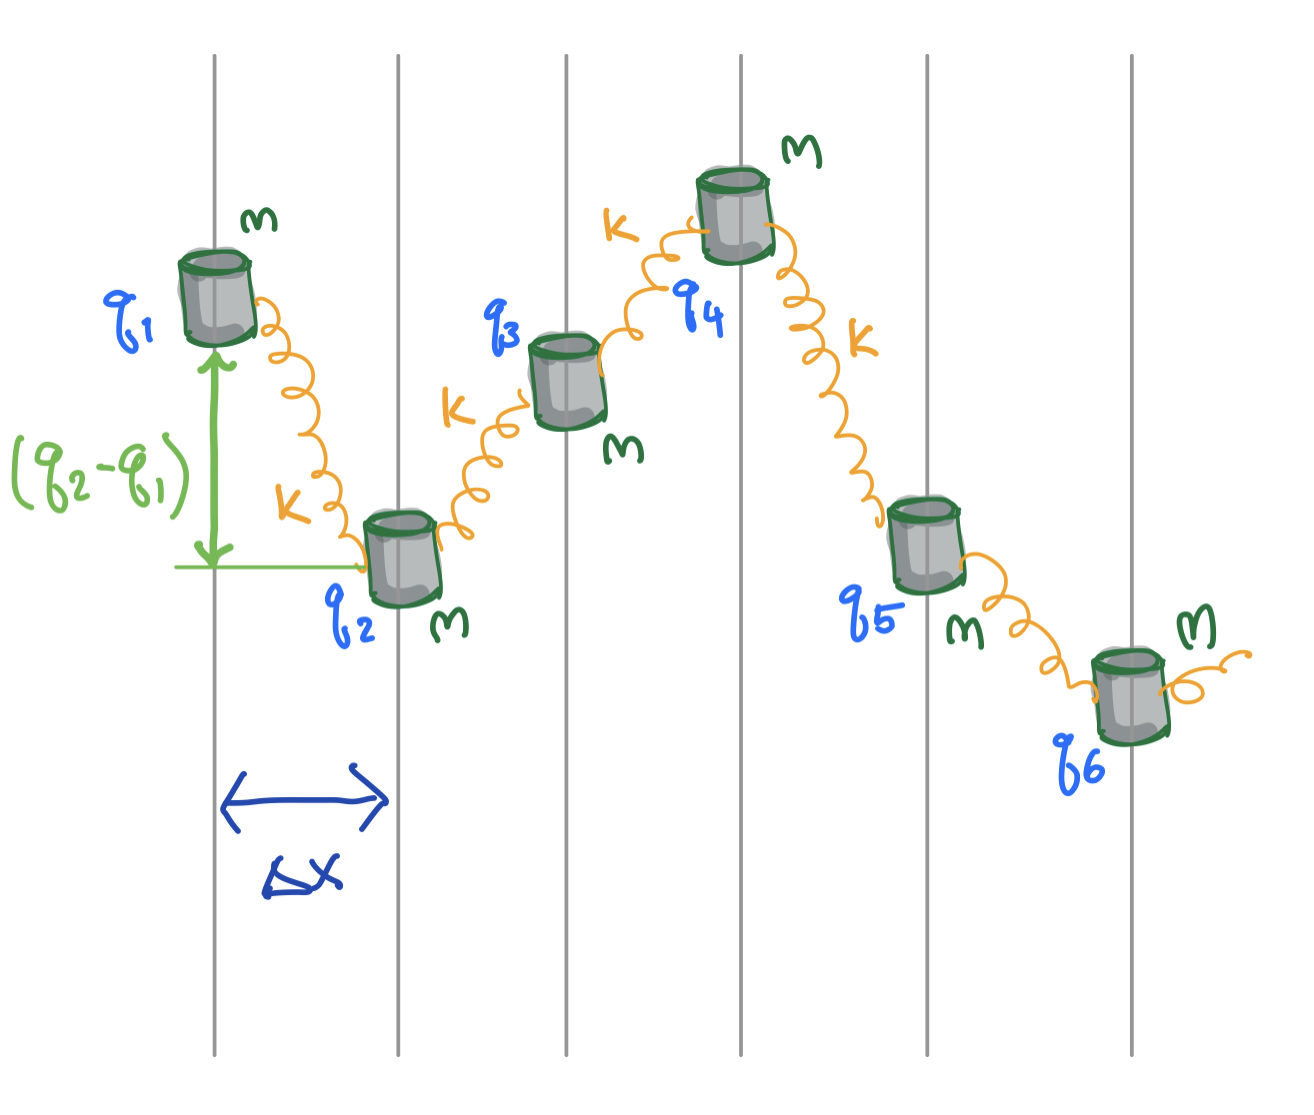
\includegraphics[width=.5\textwidth]{figures/coupledHO.jpg}
\end{center}
In the above picture we treated each value of $i$ as some point on a discretized spatial dimension. One could have equivalently treated $i$ as an index of a discretized time direction. In that way,
\begin{align}
	q_i \to q(t) \ ,
\end{align}
and the matrix/operator $A$ encodes something about propagation in time. For example, the harmonic oscillator would be $A \sim -(d/dt)^2$, where we take the appropriate discretized version of the second derivative:
\begin{align}
	A \sim 
	\begin{pmatrix}
	1 	& -2 & 1  &    &   &\\
		& 1  & -2 & 1  &   &\\
		&	 & 1  & -2 & 1 &\\
		&	&	&	&	& \ddots
	\end{pmatrix}
\end{align}
One can see clearly that $A$ couples nearby lattice points in time. If I displace the oscillator at time $i$, then at some later\footnote{One still has to impose causlity by hand since the operator is symmetric under time reversal.} time $j$ the oscillator will have some correlated displacement. In other words, the disturbance at time $i$ has \emph{propagated} to time $j$. The object that enabled that propagation is $A^{-1} \sim [-(d/dt)^2]{-1} \sim G(t,t')$. 

Observe that even though $A$ is local---the discretized second derivative connects nearest-neighbors and next-to-nearest neighbor sites---the Green's function is \emph{non}-local: it allows the information to propagate over long distances. The physical mechanism is clear: if we think about this as a bunch of coupled oscillators (in time), then each oscillator causes its neighbor to move. You should imagine `the wave' in a stadium when the crowd cheers. As a matrix, the indices of the Green's function ($A^{-1}_{ij}$) gives the value of $q_j$ given a value at $q_i$:
\begin{center}
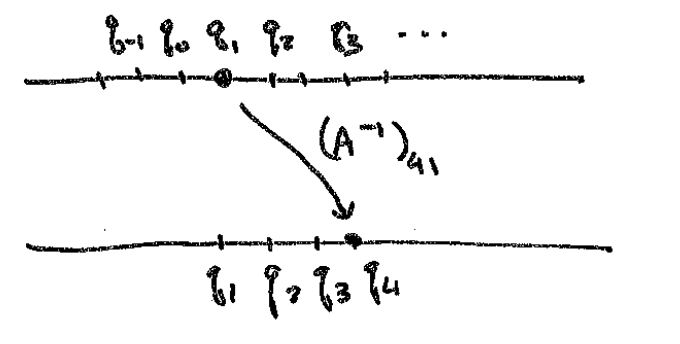
\includegraphics[width=.4\textwidth]{figures/P230b_2Ainv.png}
\end{center}
When we pass to the continuum limit, the product over $dq_1\cdots dq_N$ becomes a \emph{path integral} over all configurations in time:
\begin{align}
	\mathcal Dq(t) = dq_1\cdots dq_N \ .
\end{align}
The matrix multiplication turns into integrals
\begin{align}
	\vec{q}\vec{A}\vec{q} \to \int dt\, q(t) \left(-\frac{d^2}{dt^2} + \omega_9^2\right) q(t) \ ,
\end{align}
where you may want to take a moment to convince yourself that there's only one integral and not two. And, up to a factor of $i$, it looks like the 
\begin{align}
	Z \sim \int \mathcal Dq(t) e^{i\int dt\, L} \ ,
\end{align}
where $L$ is the harmonic oscillator Lagrangian.


In fact, we can generalize even further and go from a particle propagating in time $q(t)$ to a field propagating in spacetime $q(x,t) = \varphi(x,t)$. We just have to imagine there being more indices. We can imagine $A$ becoming a tensor that acts as a `matrix' for each direction. I say `imagine' because it's a pain in the ass to actually write out, and it's better that we just imagine that one could do this: the point is that it is conceptually simple. 
In continuum language, $A$ is simply the quadratic part of the Lagrangian density:
\begin{align}
	A\to \partial^2 = \frac{1}{c^2} \frac{\partial^2}{\partial t^2} - \nabla^2 \ ,
\end{align}
and the generating function (which I usually just call a \emph{partition function} inspired by statistical physics) is
\begin{align}
	Z &= \int \mathcal D\varphi(x,t) e^{iS[\varphi]} \ 
	&
	S[\varphi] &= \int d^4x \, \mathcal L \ ,
\end{align}
with $\mathcal L$ the Lagrangian \emph{density} for the theory. At this point, we can remind ourselves of \eqref{eq:G:QM}, throw in factors of $\hbar$ for dimensional consistency, and pat ourselves on the back. By the way, I don't think there's anything too deep to read into the fact that \eqref{eq:G:QM} is a quantum mechanical Green's function while $Z[\varphi(x,t)]$ is a partition function. There's a slight nuance related to what is called second quantization (which is related to what we've been doing), but that is now beyond the focus of this course\footnote{See, e.g.~\url{https://sites.google.com/ucr.edu/p230b/}}.

\subsection{Interpretation}

What's the lesson of all of this? The `\emph{fields are coupled harmonic oscillators in spacetime}' picture gives us a lot of intuition for solving [linear] differential equations. It brings us to the \emph{origin} of these differential equations, the action. It connects the solution to the linear differential equations to a Gaussian integral. For the non-linear cases, we still need to do some work, but this is where life gets difficult. The coupled harmonic oscillator picture also brings us back to the notion of a \emph{discretized function space} as a crutch to understand the continuum\footnote{If you're a condensed matter physicist, then the lattice holds some physical significance. If you're a particle physicist, then you assume that the lattice is just a coarse model of the continuum. In either case, you gain a lot from working with a handful of fields rather than $N\to \infty$ coupled harmonic oscillators.}. That discrete function space picture helps reinforces the idea that the Green's function is the inverse of some quadratic form\footnote{This is the fancy way of saying matrix.} in the action. 

We develop some intuition for \emph{field theory} by placing \emph{sources} $J(x,t)$ on the lattice and taking functional derivatives with respect to them. This corresponds to imagining that there's some microscopic trouble-maker jumping up and down on one the harmonic oscillator at $\varphi(x,t)$ to create excitations of the field. The Green's function transmits these excitations to the rest of the lattice, according to the dynamics $\mathcal O \sim A$. Even though the dynamics are manifestly \emph{local} (derivatives $\sim$ nearest neighbor interactions), the Green's function is a \emph{propagator} that `exponentiates\footnote{At the level of this discussion, the word `exponentiates' is not a good choice. In quantum mechanics and the representation theory of groups, however, this is literally taking infinitesimal translations in spacetime, generated by e.g.~$\hat H$, and then creating a finite transformation by exponentiating it, $e^{-i\hat H t}$. In fact, in all of what we have done, the one picture that we have `missed' is the geometric one, which I keep referring to obliquely in footnotes like this. Sometimes the real story is in the footnotes (e.g.~the novel \emph{Pale Fire}).}' microscopic interactions into long-range interactions.

\paragraph{Big Picture.}
You now have the big picture the most common differential operators in physics. You'll have to slog through all sorts of second-order differential operators that are versions of the $\partial^2$ in different coordinate systems. Sometimes you'll have differential equations that are only single derivatives in time, and you'll know that this corresponds to a non-relativistic limit. You'll know that you won't find differential operators with only one power of $\nabla$ unless the system somehow breaks translation invariance. You'll have to solve these differential equations, usually by solving for the operators' Green's functions. You can do this in multiple ways; we reviewed the most popular methods in Section~\ref{sec:ways:to:solve:G}:
\begin{enumerate}

\item \textbf{Eigenfunctions and completeness}, Section~\ref{sec:Greens:fuctions:by:completeness}. Assuming one knows the eigenfunctions of the differential operator, this gives a series solution for the Green's function. It is practically useful only when the series is convergent.

\item \textbf{Patching}, Section~\ref{sec:patching}. This method assume that one can solve the \emph{homogeneous} differential equation $\mathcal O_x G(x,x')=0$ and then produces a piece-wise solution to the \emph{inhomogeneous} differential equation that defines the Green's function, $\mathcal O_x G(x,x')=\delta(x-x')$. This is practically useful in one dimension where the boundary conditions where the pieces are connected are easy to define.

\item \textbf{Fourier transform and its cousins}. This will be the topic of the rest of our course. We convert the differential equation into an \emph{algebraic equation} in momentum space. Aspects of the causal structure of the system that are manifested in complex momentum space. Furthermore, one can use contour integrals to do the `hard work.'
\end{enumerate}
When solving the Laplacian in different coordinates, you'll have to use different basis functions in place of the Fourier transform. You'll become good friends with the Bessel functions and spherical harmonics. They may look intimidating, but you'll remember that they're just a different basis for function space and they obey all the same nice features: they are orthonormal, they have real eigenvalues, and you can project functions onto that basis. The technical work you'll have to do will be cumbersome, but you will never be lost conceptually. You can always refer back to the simpler examples in this course.

The one thing that we didn't stress in this course is actually solving physical problems. We've brought you to the point where the solution $\psi(x)$ to a differential equation $\mathcal O_x \psi(x) = s(x)$ is
\begin{align}
	\psi(x) = \int dx'\, G(x,x')\, s(x') \ .
\end{align}
Actually \emph{doing} this integral is not interesting to me. It'll be interesting to you when the differential equation has some significance in your life (e.g.~a homework problem in electrodynamics). But this is just technical work. As far as I'm concerned, you could put that integral into \emph{Mathematica} or \emph{NumPy} and get the answer. Most of the physical intuition went into writing down that integral in the first place.

Great! We're now experts in solving linear differential equations. These correspond to the quadratic parts of the action and tend to be variants of the wave operator. However, you know from Section~\ref{sec:EFT:philosophy} that there are typically \emph{more} terms in the action than the quadratic part. For example, terms that go like $\varphi^3$ or $\varphi^4$ in the action give \emph{non-linear} differential equations, $\mathcal O_\text{quad}\varphi + \lambda \phi^3 = s$, for example. We even argued that it is precisely these non-linear terms that distinguish theories from one another: otherwise they all tend to be the \emph{same} second-derivative theory of non-interacting\footnote{We say non-interacting because the plane waves that pop out of the wave equation add linearly. This is obvious, right? The whole system was linear. The result is a theory which is completely solved, but rather uninteresting.} waves. The two approaches are (1) put everything on a computer and (2) appeal to perturbation theory with respect to the non-linear terms.
 

\section{Feynman Diagrams}

The idea of Feynman diagrams is to do perturbation theory with respect to the quadratic piece of the action. Rather then jumping into the field theory language, let's keep using the more familiar $N$-site lattice language. Let the matrix $A$ represent the quadratic part of the action which, at the very least, includes the kinetic term and the nearest-neighbor interactions. There is also the linear term, $\vec{J}\vec{q}$ that we interpret as a source for $\vec{q}$. Let us add to this a quartic term which we write as
\begin{align}
 	-V(\vec{q}) &= - \lambda \sum_i q_i^4 \ .
 \end{align}
The minus sign is to remind us that this is a potential term and such terms appear with a minus sign in the Lagrangian. $\lambda$ is a number that represents the four-point coupling or interaction strength. When $q_i$ is a discrete harmonic oscillator $\lambda$ has some dimension, but upon passing to the continuum field $\varphi$ using the normalization \eqref{eq:field:normalization} one can check that $\lambda$ is dimensionless in natural units. By the way, it is important that we wrote $\sum q_i^4$ and not $(\sum_i q_i)^4$. The latter mixes terms at different sites, whereas $q_i^4$ is a local term that is evaluated at each site $i$. 

The partition function/path integral/generating function for $\vec{q}$ in the presence of $V(\vec{q})$ is
\begin{align}
	Z_V[\vec{J}] &= \mathcal N^{-1} \int d^N\vec{q} \, 
		e^{-\frac{1}{2} \vec{qAq} + \vec{Jq} - V(\vec{q})}
		\\
	&= 
	\mathcal N^{-1} \int d^N\vec{q} \, 
	e^{-V\left(\frac{\partial}{\partial \vec{J}}\right)}
		e^{-\frac{1}{2} \vec{qAq} + \vec{Jq}} \ .
\end{align}
In the second line we have used the fact that because
\begin{align}
	\mathcal N^{-1} \int d^N\vec{q} \, 
	q_i^n \, 
	e^{-\frac{1}{2} \vec{qAq} + \vec{Jq}}
	=
	\mathcal N^{-1} \int d^N\vec{q} \, 
	\left(\frac{\partial}{\partial J_i}\right)^n
	e^{-\frac{1}{2} \vec{qAq} + \vec{Jq}} \ ,
\end{align}
one may write any function of $q_i$, including $e^{-V(\vec{q})}$ as a function of $(\partial/\partial J_i)$ acting on $Z[J]$, the generating function \emph{without} $V(\vec{q})$. Thus
\begin{align}
	Z_V[\vec{J}] &= e^{-V\left(\frac{\partial}{\partial \vec{J}}\right)} Z[\vec{J}] \ .
	\label{eq:ZV:from:Z}
\end{align}
It is conventional to write the generating function(al) to be a function of the source $\vec{J}$ since it is formally an integral transform of the distribution. When we take correlation functions, we take derivatives of $Z_V[\vec{J}]$ with respect to $\vec{J}$, recall \eqref{eq:correlator:J}.

As long as $\lambda$ is small, one may Taylor expand the exponential in $V(\vec{q})$,
\begin{align}
	Z_V[\vec{J}] &= Z[\vec{J}] + \lambda\left[-\sum_i \left(\frac{\partial}{\partial J_i}\right)^4\right] Z[\vec{J}] + \cdots \ .
\end{align}

Let's put this to work. Suppose I'd like to ask about the four-point correlation function between four oscillators, which I'll call $q_{1,2,3,4}$. I'm labeling them 1--4 for notational simplicity, not because they have to be sequential oscillators. You could have picked any four numbers, say $q_4$, $q_9$, $q_{8}$, and $q_{24}$. Mathematically, we know what this object corresponds to:
\begin{align}
	\langle q_1q_2q_3q_4 \rangle
	&= 
	\frac{1}{\mathcal N}
	\int d^N\vec{q} \, 
	q_1q_2q_3q_4 \,
	e^{-\frac{1}{2}\vec{qAq} - V(\vec{q})}
	\\
	&=
	\left.\frac{\partial^4 Z_V[\vec{J}]}{\partial J_1\partial J_2\partial J_3 \partial J_4}\right|_{\vec{J}=0}
	\\
	&= \left.\partial_{J_1}\partial_{J_2}\partial_{J_3}\partial_{J_4}
	\left(1 - \lambda\sum_i \partial_{J_i}^4 + \cdots\right) Z[\vec{J}] 
	\right|_{\vec{J}=0}
	\ .
	\label{eq:4pt:example:4derivatives}
\end{align}
At this point, let us recall the closed form expression for $Z[\vec{J}]$ from performing the Gaussian integral, \eqref{eq:Z:gaussian}:
\begin{align}
	Z[\vec{J}]
	=
	e^{\frac{1}{2}\vec{J}\vec{A}^{-1}\vec{J}} \ .
\end{align}
This means that
\begin{align}
	\left.
	\partial_{J_k}Z[\vec{J}]
	\right|_{\vec{J}=0}
	&= 
	\left(\vec{A}^{-1}\vec{J}\right)_k
	= 0
	&
	\left.
	\partial_{J_k}\partial_{J_\ell}Z[\vec{J}]
	\right|_{\vec{J}=0}
	&= 
	A^{-1}_{k\ell}
	\ .
\end{align}
This means that every \emph{pair} of derivatives with respect to source lattice sites $J_k$ and $J_\ell$ produces a propagator (Green's function) $A^{-1}_{k\ell}$. Any single derivative $\partial_{J_k}$ of $Z$ is proportional to $A^{-1}J$, which vanishes when we set the sources to zero. The $\mathcal O(\lambda^0)$ term of \eqref{eq:4pt:example:4derivatives} may be written as:
\begin{align}
	\left.
	\partial_{J_1}\partial_{J_2}\partial_{J_3}\partial_{J_4}
	Z[\vec{J}] 
	\right|_{\vec{J}=0}
	&=
	A^{-1}_{12}A^{-1}_{34} + A^{-1}_{13}A^{-1}_{24} + A^{-1}_{14}A^{-1}_{23} \ .
	\label{eq:4pt:ex:4der:leading:props}
\end{align}
The indices refer to particular lattice points where the sources are turned on. These, in turn, correspond to the specific oscillators int he correlation function $\langle q_1q_2q_3q_4 \rangle$. 
\begin{exercise}
Check that \eqref{eq:4pt:ex:4der:leading:props} is correct. You may need to do this the hard way and write out a bunch of terms to see how it works out. It is worth your time doing this to see how \eqref{eq:4pt:ex:4der:leading:props} pops out. 
\end{exercise}
There is a graphical way of drawing this. Assign each point $i=1,2,3,4$ a point on the page and draw $A^{-1}_{k\ell}$ as a line that connects point $k$ to point $\ell$. The result is
\begin{align}
	A^{-1}_{12}A^{-1}_{34} + A^{-1}_{13}A^{-1}_{24} + A^{-1}_{14}A^{-1}_{23} 
	&=
	\vcenter{
		\hbox{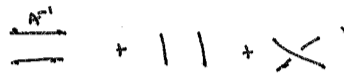
\includegraphics[width=.4\textwidth]{figures/P230b_4ptdisco.png}}
		} \ .
\end{align}
The $\mathcal O(\lambda)$ term now has \emph{eight} derivatives with respect to $\vec{J}$; the four new ones are at some \emph{new} point $J_i$, which is then summed over: 
\begin{align}
	\left.
		- \lambda\sum_i
		\partial_{J_1}\partial_{J_2}\partial_{J_3}\partial_{J_4}
		 \partial_{J_i}^4
		Z[\vec{J}] 
	\right|_{\vec{J}=0} \ .
\end{align}
Following our observation above that pairs of $\partial_{J_k}\partial_{J_\ell}$ bring down a propagator $A^{-1}_{k\ell}$, we can write this diagrammatically in terms of a general intermediate point $i$ that is summed over:
\begin{align}
	\left.
		- \lambda\sum_i
		\partial_{J_1}\partial_{J_2}\partial_{J_3}\partial_{J_4}
		 \partial_{J_i}^4
		Z[\vec{J}] 
	\right|_{\vec{J}=0} 
	&=
	- 4! \lambda \sum_i
	A^{-1}_{1i} A^{-1}_{2i} A^{-1}_{3i} A^{-1}_{4i} \ .
\end{align}
The $4!$ is a combinatorial factor that counts the number of different ways in which you can pair up $J_i$ derivatives with $J_{1,2,3,4}$ derivatives. 
\begin{exercise}
Confirm the factor of $4!$ by explicitly deriving the above result.
\end{exercise}
Finally, we may write this diagrammatically as well:
\begin{align}
	- 4! \lambda \sum_i
	A^{-1}_{1i} A^{-1}_{2i} A^{-1}_{3i} A^{-1}_{4i}
	&= 
	\vcenter{
		\hbox{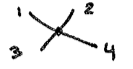
\includegraphics[width=.2\textwidth]{figures/P230b_4ptlocal.png}}
		}\ .
\end{align}
What we end up with is a rule for describing the Taylor expansion of $e^{-V[\partial_{\vec{J}}]}$ in \eqref{eq:ZV:from:Z} when calculating $n$-point correlation functions $\langle q_1\cdots q_n\rangle$:
\begin{enumerate}
\item For each of the $n$ points, draw a point on the page. Your goal will be the connect these points into a graph.

\item To leading order, connect all the points using lines that do not intersect. This represents free propagation and is the $\mathcal O(\lambda^0)$ contribution.

\item The $\mathcal O(\lambda)$ graphs correspond to the same set up, but with one additional point that accepts four lines. Draw all graphs where each point is connected, with the reminder that the new point must have four lines connecting to it.

\item You can read this graph as the product of propagators $A^{-1}_{k\ell}$ corresponding to each line. Each four-point vertex picks up a factor $\lambda$ (up to other combinatorial factors that one may determine).

\item For higher-order terms, you insert more vertices that accept four lines. One such vertex for each order in $\lambda$. You interpret more complicated diagrams the same way: each line corresponds to a propagator between those two nodes, each vertex comes with a prefactor of $\lambda$ up to combinatorial factors.
\end{enumerate}
As long as $\lambda$ is small, one may truncate the sum at a small number of insertions to approximate the correlation function. These are called Feynman diagrams.

Note that each line is a Green's function from the \emph{quadratic} operator $\vec{qAq}$: each line represents the solution to the \emph{linear} differential equation. Recall that this Green's function is precisely what `propagates' over long distances as a free wave. The vertices are the non-linearities. You can see this because rather than one $q$ coming in and one $q$ coming out, you have many $q$'s interacting at the same point. For example, you could read this as one $q$ turning into three lower-energy $q$s. This non-conservation of particle number for an interacting theory is part of what makes a quantum theory of fields different from quantum mechanics. 

The sum over all of these Feynman diagrams is completely analogous to the sum over histories in quantum mechanics. You can imagine that $q_1$ and $q_2$ are some harmonic oscillators in in the asymptotic past that have excitations. We would like to know the amplitude for those excitations to show up at harmonic oscillators $q_3$ and $q_4$ in the asymptotic future. In order to figure that out, we sum over all the ways in which those excitations could propagate. The leading terms include no interactions; this term is usually zero since you can't exchange momentum. The next-to-leading terms include an interaction where the initial particles overlap at a point $q_i$ before spitting out two new particles. In this way, you can `read off' a story of what the excitations are doing in spacetime. Now you know everything you need to know to play with Feynman diagrams\footnote{See, e.g.~\url{https://sites.google.com/ucr.edu/p165/}. For a teaser, you can try this exercise that I give to the undergraduate particle physics course: \url{https://github.com/Tanedo/Physics165-2020/blob/master/P165_L02.pdf}.}.








 





% Connected: https://www.youtube.com/watch?v=7WaBFvjk06w
% Then: do bayes
% Tenn: do Kramers Kronig










